% \documentclass[AMA,Times1COL]{WileyNJDv5}
\documentclass[HARVARD,LATO2COL]{WileyNJDv5}


\articletype{Article Type}%

\received{Date Month Year}
\revised{Date Month Year}
\accepted{Date Month Year}
\journal{Journal}
\volume{00}
\copyyear{2023}
\startpage{1}

\raggedbottom
\usepackage{graphicx}
\usepackage{tikz}
\usetikzlibrary{positioning,arrows.meta}
\usepackage{booktabs}
\usepackage{multirow}
\usepackage{listings}
\usepackage{url,overcite}
\usepackage{xcolor}
% Command to mark revised text for professor review
\newcommand{\rev}[1]{\textcolor{red}{#1}}


\begin{document}

\title{AN AIOT-Based Alcohol Level Detection and Vehicle Ignition Prevention System}

\author[1]{Anastasiia Igorevna Shaposhnikova}
\author[1]{Sudhanshu Tripathi}
\author[1]{Ram Naresh}
\author[2]{Pramod Kumar Soni}
\author[3]{Shikha Chaudhary}

\authormark{SHAPOSHNIKOVA \textsc{et al.}}
\titlemark{AN AIOT-BASED ALCOHOL LEVEL DETECTION AND VEHICLE IGNITION PREVENTION SYSTEM}

\address[1]{\orgdiv{Department of Information Technology}, \orgname{Amity University Tashkent}, \orgaddress{\state{Tashkent}, \country{Uzbekistan}}}
\address[2]{\orgdiv{Department of Computer Applications}, \orgname{Manipal University Jaipur, Jaipur}, \orgaddress{\state{Rajasthan}, \country{India}}}
\corres{Pramod Kumar Soni \email{pramod.soni@jaipur.manipal.edu}}

\address[3]{\orgdiv{Department of IT}, \orgname{Manipal University Jaipur, Jaipur}, \orgaddress{\state{Rajasthan}, \country{India}}}

%\presentaddress{}

%\fundingInfo{Text}
%\JELinfo{ejlje}

\abstract[Abstract]{\textcolor{red}{\textbf{Introduction/Objective:} Alcohol-impaired driving accounts for 28\% of U.S. traffic fatalities, yet existing ignition interlocks rely on breath sampling that drivers can circumvent. This paper presents PhysioWatch-BAC, a wearable-to-vehicle system that passively estimates blood alcohol concentration and enforces fail-safe ignition control without requiring driver interaction.
\textbf{Methods:} PhysioWatch-BAC fuses photoplethysmography, electrodermal activity, and skin temperature from a Wear OS smartwatch through a bidirectional long short-term memory network with learned temporal attention. Training uses an asymmetric loss function that penalizes false negatives 5$\times$ more heavily than false positives. The quantized TensorFlow Lite model communicates 20-byte status packets to an Arduino Nano 33 BLE vehicle controller. Region-specific climate calibration coefficients compensate for ambient temperature and humidity variation.
\textbf{Results:} Hardware-in-the-loop simulation on synthetic physiological sequences yielded 0.0082~g/dL mean absolute error, 97.3\% classification accuracy at the 0.08~g/dL legal threshold, 0.7\% false negative rate, and 580~ms end-to-end latency. The deployed model occupies 22~KB with 42~ms inference time per prediction.
\textbf{Discussion:} These results place PhysioWatch-BAC within 15\% of clinical transdermal monitors at a fraction of the cost, while the asymmetric loss design prioritizes the safety-critical suppression of missed intoxication events.
\textbf{Conclusion:} The system establishes feasibility of continuous, passive alcohol monitoring for vehicle safety with fail-safe ignition blocking under communication loss, watch removal, or stale data conditions.}}

\keywords{blood alcohol concentration, \rev{wearable biosensor, sensor fusion, deep learning, TinyML, ignition interlock,} Bluetooth Low Energy\rev{, vehicle safety}}

\jnlcitation{\cname{%
\author{Shaposhnikova A.I.},
\author{Tripathi S.},
\author{Naresh R.}, and
\author{Soni P.K.}}.
\ctitle{AN AIOT-Based Alcohol Level Detection and Vehicle Ignition Prevention System.} \cjournal{\it J Comput Sci Cybern.} \cvol{2026;00(00):1--6}.}


\maketitle

\renewcommand\thefootnote{}
\footnotetext{\textbf{Abbreviations:} BAC, blood alcohol concentration; BLE, Bluetooth Low Energy; BiLSTM, Bidirectional Long Short-Term Memory; PPG, photoplethysmography; EDA, electrodermal activity; FSM, finite state machine.}

\renewcommand\thefootnote{\fnsymbol{footnote}}
\setcounter{footnote}{1}

\section{Introduction}\label{sec1}

\rev{Alcohol-impaired driving kills. In the United States alone, 28\% of traffic fatalities involve alcohol~\citep{nhtsa2022}; globally, the WHO attributes 1.35 million annual road deaths to related causes~\citep{who2018}. Legislation sets BAC thresholds---typically 0.08~g/dL---but enforcement remains sporadic. Breathalyzer checkpoints cover a fraction of road segments at predictable times, and motivated drivers route around them~\citep{das2023, lombardo2020l}. This gap between policy and practice has driven interest in passive, continuous monitoring systems that pair wearable biosensors with vehicle control~\citep{watchover}.}

\rev{The existing technology landscape has clear shortcomings. Breathalyzer-based ignition interlocks, documented in U.S. Patents 5,736,965 and 7,113,834~\citep{uspat5736965, uspat7113834} and Indian Patent 286703~\citep{inpat286703}, require the driver to consciously provide a breath sample. A sober passenger can blow on behalf of the driver; the device cannot tell the difference. Vanlaar et al.~\citep{interlock2024} confirmed through a discrete choice experiment that interlock penalties carry real deterrent weight, but the bypass problem undermines their effectiveness. Single-modality wearable sensors offer passive detection---no breath sample needed---yet they struggle with accuracy when ambient conditions change or when physiological variation across individuals widens the error bars~\citep{bush2024development}. Transdermal alcohol sensing through skin ethanol diffusion avoids the participation problem, but the signal is weak and delayed~\citep{fairbairn2021, fairbairn2025}. Systematic reviews confirm that wearable transdermal devices detect drinking events reliably in the lab, less so in the field~\citep{wang2022jmir, tay2023}.}

\rev{Two converging trends make a new approach feasible. First, edge AI has matured: TinyML frameworks now run meaningful neural models on ARM Cortex-M processors with milliwatt power budgets~\citep{zhou2025tinyml, abadade2023}, and IoT-enabled deep learning has been validated for real-time health monitoring~\citep{wu2023internet}.} Verg\’{e}s et al.~\citep{verges2024} \rev{applied hyperdimensional computing to smartwatch-based BAC prediction with promising accuracy, though the computational overhead limits always-on deployment. Second,} multimodal sensor fusion---combining heart rate variability, skin conductance, and temperature\rev{---provides richer input than any individual channel}~\citep{sensors2024, sensors2023, vedanarayanan2024}. \rev{ML-based BAC estimation has been attempted through diverse modalities: smart-breathalyzer behavioral signatures~\citep{gharani2021}, smartphone accelerometer gait analysis~\citep{killian2019}, and smartwatch-based ecological momentary assessment}~\citep{alcowatch2025}. \rev{Chen et al.~\citep{chen2025} recently validated PPG-based alcohol impairment detection using ensemble learning, confirming that wrist-worn optical sensors carry usable alcohol-related signal.}

\rev{What is missing is integration. Each of these works addresses one piece---sensing, estimation, or vehicle control---in isolation. No existing system combines multimodal wearable inference, fail-safe ignition blocking, and climate-adaptive calibration in a single pipeline. Building one that fits within the 22~KB memory and 50~ms latency budget of a consumer smartwatch is the challenge this paper addresses.}
\par
\begin{figure*}[t]
\centering
\begin{tikzpicture}[
  node distance=0.3cm and 0.4cm,
  >=Latex,
  font=\scriptsize,
  block/.style={draw, rounded corners=2pt, align=center, text width=1.6cm, minimum height=0.65cm, inner sep=2pt, line width=0.4pt},
  sensor/.style={block, fill=blue!8},
  proc/.style={block, fill=green!8},
  comm/.style={block, fill=orange!8},
  vehicle/.style={block, fill=red!8},
  group/.style={draw, dashed, rounded corners=4pt, inner sep=4pt, line width=0.3pt, gray},
  link/.style={->, line width=0.5pt},
  datalabel/.style={font=\tiny, text=gray, midway, above, sloped},
]

% === Wear OS Smartwatch ===
% Sensor layer
\node[sensor] (ppg) {PPG\\(64 Hz)};
\node[sensor, right=of ppg] (eda) {EDA\\(estimated)};
\node[sensor, right=of eda] (temp) {Skin Temp\\Ambient};

% Processing layer
\node[proc, below=0.5cm of eda] (feat) {Feature\\extraction};
\node[proc, below=0.4cm of feat] (lstm) {BiLSTM +\\Attention};
\node[proc, right=of lstm] (cal) {Climate\\calibration};

% Group: Smartwatch
\node[group, fit=(ppg)(eda)(temp)(feat)(lstm)(cal), label={[font=\tiny\bfseries]above:Wear OS Smartwatch}] (watch) {};

% === BLE Communication ===
\node[comm, right=1.0cm of cal] (ble) {BLE GATT\\(20 bytes)};

% === Arduino Vehicle Module ===
\node[vehicle, right=1.0cm of ble] (fsm) {Ignition\\FSM};
\node[vehicle, above=0.3cm of fsm] (parse) {Packet\\validation};
\node[vehicle, below=0.3cm of fsm] (relay) {Relay\\control};

% Group: Arduino
\node[group, fit=(parse)(fsm)(relay), label={[font=\tiny\bfseries]above:Arduino Nano 33 BLE}] (arduino) {};

% === Output ===
\node[block, fill=gray!10, right=0.5cm of relay] (ign) {Ignition\\allow/block};

% === Arrows ===
\draw[link] (ppg) -- (feat);
\draw[link] (eda) -- (feat);
\draw[link] (temp) |- (feat);
\draw[link] (feat) -- (lstm);
\draw[link] (lstm) -- node[datalabel] {BAC} (cal);
\draw[link] (cal) -- node[datalabel] {status} (ble);
\draw[link] (ble) -- (parse);
\draw[link] (parse) -- (fsm);
\draw[link] (fsm) -- (relay);
\draw[link] (relay) -- (ign);

% Data annotations
\node[font=\tiny, text=gray, below=0.1cm of lstm] {22 KB TFLite};
\node[font=\tiny, text=gray, below=0.05cm of ble] {AES-256, 30s};

\end{tikzpicture}

\caption{Architecture and data flow of the proposed system.}
\label{fig:system}
\end{figure*}

\begin{figure*}[t]
\centering
\input{sequence_diagram.tikz}
\caption{Operational sequence from sensing to ignition control.}
\label{fig:sequence}
\end{figure*}
\rev{This paper introduces PhysioWatch-BAC, an integrated wearable-to-vehicle system that passively estimates BAC from multimodal physiological signals and enforces fail-safe ignition control without requiring driver interaction. The architecture bridges smartwatch biosensing with automotive safety through lightweight on-device inference and secure BLE communication. Key contributions include:}
\begin{enumerate}
    \item \rev{A multimodal sensor fusion approach combining PPG, EDA, and temperature signals with a BiLSTM-attention architecture for continuous BAC estimation on a Wear OS smartwatch.}
    \item \rev{A safety-prioritized asymmetric loss function with 5$\times$ false negative penalty, achieving sub-1\% false negative rate while maintaining low false positive rate.}
    \item \rev{Climate-adaptive calibration with region-specific coefficients that maintain estimation accuracy across diverse ambient conditions ($-$20$^\circ$C to 50$^\circ$C).}
    \item \rev{A secure BLE communication protocol with fail-safe timeout mechanisms and continuous watch-wear verification.}
    \item \rev{A vehicle-side finite state machine that guarantees ignition blocking under communication loss, watch removal, or stale data conditions.}
\end{enumerate}
\section{Related Work} \label{sec21}
% === ALL CONTENT BELOW UNTIL \section{Methodology} IS NEW ===
{\color{red}% BEGIN REVISED RELATED WORK

\subsection{Alcohol Detection via Physiological Signals}
Transdermal alcohol monitoring bypasses the need for breath sampling by measuring ethanol diffusing through the skin. The approach is not new---SCRAM ankle monitors have been court-mandated for over a decade---but wrist-worn consumer devices are a recent development. A systematic review by Wang et al.~\citep{wang2022jmir} covering 23 studies found that while existing transdermal sensors reliably detect drinking episodes in controlled settings, accuracy drops sharply in the field. Tay et al.~\citep{tay2023} put numbers to this gap: commercially available monitors exhibit MAE of 0.015--0.032~g/dL under laboratory conditions, well above the precision needed for legal BAC thresholds.
The picture is improving. Fairbairn et al.~\citep{fairbairn2025} collected over 5.39~million transdermal readings from 100 participants wearing rapid-sampling wrist sensors (20-second intervals) across both lab sessions and 14-day field deployments. Their ML pipeline yielded AUROC of 0.966 for drinking detection---encouraging, but the underlying TAC-to-BAC conversion still introduces lag and individual variability. Sirlanci et al.~\citep{sirlanci2019} tackled this mapping with a population-based deconvolution model; the mathematical elegance comes at a computational cost that rules out on-device execution.
On the clinical side, transdermal sensors are proving useful beyond enforcement. Karns-Wright et al.~\citep{karns-wright2025} deployed them for post-detoxification monitoring with contingency management, while Hahn et al.~\citep{hahn2023} showed in a JAMA study that continuous wearable sensing captures drinking patterns that periodic phosphatidylethanol biomarkers simply miss. The gap that remains: achieving BAC-level accuracy on a consumer smartwatch without dedicated alcohol-specific hardware.

\subsection{Wearable Sensor Fusion for Physiological Monitoring}
A single sensor tells an incomplete story. PPG alone cannot distinguish elevated heart rate from alcohol versus exercise; EDA spikes may reflect thermal stress rather than sympathetic activation from intoxication. Fusing multiple modalities mitigates these ambiguities. Mejia-Trujillo et al.~\citep{mejia2024} showed this concretely: combining PPG, EDA, and accelerometry lifted activity recognition accuracy well above any single-channel baseline, with the EDA channel providing discriminative power precisely in the low-motion states where accelerometers contribute little.
From the cardiovascular perspective, Saarela et al.~\citep{saarela2025} reviewed current wearable sensor capabilities and noted that PPG-derived heart rate variability (HRV) and pulse wave morphology track autonomic nervous system shifts---the same physiological axis that alcohol consumption perturbs. Reiss et al.~\citep{reiss2019} pushed further by applying deep CNNs directly to raw PPG waveforms, achieving heart rate estimation errors below 5~bpm even during vigorous activity. This matters for our design: robust heart rate extraction under motion artifacts is a prerequisite for BAC-correlated feature extraction.
Li et al.~\citep{li2025multitask} introduced a multitask framework that simultaneously evaluates PPG signal quality and estimates physiological parameters---a joint optimization that maps naturally onto our architecture, where sensor confidence scores weight the BAC prediction. Still, none of these fusion studies target alcohol specifically, and none address the downstream question of what to do with the estimate (i.e., vehicle control).

\subsection{Machine Learning for BAC Estimation}
ML-based alcohol detection has been attempted through remarkably diverse input modalities. Gharani et al.~\citep{gharani2021} extracted behavioral features from how users interact with a smart breathalyzer---blow duration, device handling patterns---and predicted BAC with 0.87 AUC using gradient-boosted trees. The catch: users must actively blow into the device. Killian et al.~\citep{killian2019} avoided this by training on smartphone accelerometer data, detecting heavy drinking episodes at 77.5\% accuracy from gait patterns alone. Suffoletto et al.~\citep{suffoletto2020} pursued a similar accelerometer-based strategy for impaired driving detection. Both studies confirm an important point---motion-based sensing captures gross impairment but lacks the resolution for quantitative BAC estimation.
Neural architectures offer more precision. Kong et al.~\citep{kong2024} paired a bidirectional LSTM with CNN on remote PPG signals for fatigue detection, finding that temporal attention markedly improved the network's ability to track physiological state transitions across time. This result influenced our choice of BiLSTM with learned attention weights. Kim et al.~\citep{kim2024eeg} applied LSTM networks to alcoholic EEG classification with LASSO-based feature selection, reinforcing that recurrent architectures handle the temporal dynamics of alcohol's physiological effects well.
Two recent studies are particularly relevant. Saeed et al.~\citep{saeed2025} benchmarked five classifiers---Transformer, BiLSTM, GRU, 1D-CNN, and hyperdimensional computing (HDC)---on three weeks of smartwatch data combining TAC, accelerometer, gyroscope, and heart rate. HDC won on efficiency; BiLSTM on raw accuracy. Their finding that model size and inference cost matter as much as predictive performance on wearable hardware directly validates our design emphasis on a 22~KB TFLite footprint. Campbell et al.~\citep{biosensor2025nonwear} tackled a different practical problem: detecting when the alcohol biosensor is not being worn. Their random forest classifier achieves 0.96 sensitivity for non-wear detection, a capability we implement through continuous skin-contact verification on the watch side.

\subsection{Vehicle Ignition Interlock Systems}
Ignition interlock devices (IIDs) work. Vanlaar et al.~\citep{interlock2024} found through a discrete choice experiment ($n=583$) that a one-year interlock penalty deters drunk driving as effectively as a \$2,000 fine increase. The need is clear: NHTSA reports 28\% of U.S. traffic fatalities involve alcohol~\citep{nhtsa2022}, and the WHO~\citep{who2018} attributes 1.35 million annual road deaths globally to related causes.
Yet current IIDs share a fundamental weakness. Every commercial system requires the driver to blow into a mouthpiece---a conscious act that can be delegated, timed around, or simply refused until sober enough to pass~\citep{das2023, vedanarayanan2024}. Kumar et al.~\citep{kumar2023} integrated an MQ-3 gas sensor with an Arduino-based ignition lock, adding IoT connectivity, but the core limitation persists: the sensor must be near the driver's breath. Kommey et al.~\citep{kommey2022} designed a smart vehicle ignition interlock with additional biometric verification, though their prototype similarly depends on proximity-based alcohol detection rather than continuous monitoring.
A different line of work explores passive physiological sensing as an alternative. AlArnaout et al.~\citep{alarnaout2025} used HRV features from wearable sensors to detect driver drowsiness, and Siam et al.~\citep{siam2023} classified driver stress from non-invasive physiological signals using ML. Neither targets BAC estimation directly, but both confirm that wearable physiological data carries sufficient signal for impairment-related classification. PhysioWatch-BAC closes this loop: passive BAC estimation feeds a vehicle-side FSM that defaults to ignition blocking, removing the conscious participation requirement entirely.

\subsection{On-Device ML for Wearable Devices}
A Wear OS smartwatch is not a GPU cluster. The Cortex-M4 in an Arduino Nano 33 BLE has 256~KB of SRAM; the application processor in a typical smartwatch offers somewhat more, but thermal throttling and battery life impose hard limits. Fitting a useful deep learning model into this envelope is a well-studied problem. Zhou et al.~\citep{zhou2025tinyml} surveyed the progression from TinyML to what they term ``Tiny Deep Learning,'' covering quantization, pruning, and neural architecture search. Ray~\citep{ray2022} established the theoretical foundations earlier, framing TinyML as its own paradigm distinct from conventional edge computing.
On the practical side, Abadade et al.~\citep{abadade2023} benchmarked TensorFlow Lite Micro and found that 8-bit post-training quantization consistently delivers 3--4$\times$ size reduction with negligible accuracy degradation---a result we rely on for our Float16 quantization pipeline. Osman and Samara~\citep{osman2024} cataloged TinyML deployments across IoT verticals, identifying health monitoring as the fastest-growing application area. Two domain-specific studies stand out: Mughal et al.~\citep{mughal2025} confirmed that LSTM-based cardiac monitoring models run successfully on wearable-class processors, and Abu-Samah et al.~\citep{abusamah2025} deployed stress classification on a constrained wearable, reporting that the primary bottleneck was memory allocation for intermediate activations rather than raw compute.
Our model fits comfortably within these constraints: 22~KB after quantization, 42~ms inference, 2.3~MB peak memory. The attention mechanism adds roughly 3~KB to the LSTM-only baseline but improves MAE by 32\%---a worthwhile trade at this model scale.

\subsection{BLE Communication for Safety-Critical IoT}
BLE was designed for hearing aids and fitness trackers, not vehicle ignition control. The protocol trades security for power efficiency by design~\citep{lonzetta2018}, which creates tension when the communication channel carries safety-critical BAC data. G{\'o}mez et al.~\citep{gomez2025} charted BLE's evolution through version 6.0, which introduced channel sounding for centimeter-accurate distance measurement and phase-based ranging to defeat relay attacks---capabilities originally driven by automotive keyless entry but equally applicable to wearable-to-vehicle links.
The threat landscape is well-documented. Zuo et al.~\citep{zuo2022} identified eavesdropping, man-in-the-middle, and replay attacks as the primary BLE vulnerabilities in IoT and wearable contexts, recommending GATT-level encryption as a minimum countermeasure. Wu et al.~\citep{wu2023bleguide} went further, building automated tools that found many production IoT apps fail to validate GATT characteristic permissions at all---a sobering result for any safety-critical BLE application.
Our protocol addresses these concerns through layered defenses rather than relying on BLE pairing alone. Each 20-byte BAC status packet includes a 5-byte MAC field for message authentication (with AES-256-GCM planned for production deployment). The 60-second timeout mechanism blocks ignition if no valid packet arrives, defending against both accidental disconnects and deliberate jamming.

\subsection{Summary}
Table~\ref{tab:comparison} positions PhysioWatch-BAC against representative existing approaches. The most recent comparable work by Kaura and Joshi~\citep{kaura2025} reported 98.99\% accuracy using MLP with PPG, TAS, and GSR fusion, but relies on cloud-based processing and lacks vehicle integration. Kommey et al.~\citep{kommey2022} implemented a smart vehicle ignition interlock but without wearable sensing. While prior work has addressed individual aspects---transdermal sensing, ML-based BAC estimation, or vehicle interlock control---no existing system integrates all three within a wearable-to-vehicle pipeline that includes multimodal on-device inference, fail-safe ignition control, and climate-adaptive calibration.

\begin{table*}[t]
\caption{Comparison of PhysioWatch-BAC with Existing Approaches}
\label{tab:comparison}
\centering
\small
\resizebox{\textwidth}{!}{%
\begin{tabular}{@{}lccccccccc@{}}
\toprule
\textbf{Feature} & \textbf{Fairbairn} & \textbf{Verg\'{e}s} & \textbf{Gharani} & \textbf{Kaura} & \textbf{Kumar} & \textbf{Killian} & \textbf{Saeed} & \textbf{Trad. IID} & \textbf{Ours} \\
 & \textbf{\citep{fairbairn2025}} & \textbf{\citep{verges2024}} & \textbf{\citep{gharani2021}} & \textbf{\citep{kaura2025}} & \textbf{\citep{kumar2023}} & \textbf{\citep{killian2019}} & \textbf{\citep{saeed2025}} & & \\
\midrule
Sensing modality & TAC & TAC & Behavioral & PPG+TAS+GSR & MQ-3 gas & Accel. & Multi-sensor & Breath & PPG+EDA+Temp \\
Passive monitoring & Yes & Yes & No & Yes & No & Yes & Yes & No & Yes \\
On-device ML & No & Yes & No & Cloud & No & No & Yes & N/A & Yes (22~KB) \\
BAC estimation & Indirect & Yes & Yes & Yes & Binary & No & No & Direct & Yes \\
Vehicle integration & No & No & No & No & Yes & No & No & Yes & Yes \\
Fail-safe FSM & N/A & N/A & N/A & N/A & No & N/A & N/A & Partial & Yes \\
Climate calibration & No & No & No & No & No & No & No & No & Yes \\
Real-time ($<$1s) & No & Yes & No & No & Yes & No & Yes & Yes & Yes (580~ms) \\
\bottomrule
\end{tabular}
}
\end{table*}

}% END REVISED RELATED WORK

\section{Methodology}\label{sec2}
PhysioWatch-BAC is divided into three hardware components: the Wear OS smartwatch running the sensor reading and neural network inference, the Arduino Nano 33 BLE module running the ignition relay control, and the custom BLE GATT service handling the encrypted status transfer. Figure~\ref{fig:system} illustrates this distributed topology.
From the computational perspective, the smartwatch performs the $O(n^2)$ attention and BiLSTM passes, and the Arduino performs the deterministic FSM with $O(1)$ transitions. This is achieved while keeping the power consumption below 35~mW and the decision time below 10~ms. Figure~\ref{fig:sequence} traces the end-to-end data path. Processing proceeds as:
\begin{enumerate}
    \item Physiological sensors (PPG, EDA, temperature) capture raw signals at 64 Hz
    \item Signal processing algorithms extract features and remove noise
    \item TensorFlow Lite model performs BAC inference on 10-timestep sequences
    \item Climate-adaptive calibration adjusts estimates for environmental conditions
    \item BLE peripheral broadcasts 20-byte status packets every 30 seconds
    \item Arduino BLE central receives and validates packet integrity
    \item Ignition control state machine makes enable/disable decisions
    \item Visual and audio feedback provides driver notifications
\end{enumerate}
\subsection{PhysioWatch-BAC Neural Network Architecture}
The proposed PhysioWatch-BAC model employs a temporal sequence processing architecture that combines Bidirectional Long Short-Term Memory (BiLSTM) networks with a learned attention mechanism for BAC regression. Table~\ref{tab:model_arch} details the network configuration.
\begin{table}[htbp]
\caption{Neural Network Architecture Specifications}
\label{tab:model_arch}
\centering
\small
\begin{tabular}{@{}lll@{}}
\toprule
\textbf{Layer} & \textbf{Configuration} & \textbf{Output Shape} \\
\midrule
Input & 10 timesteps $\times$ 6 features & [batch, 10, 6] \\
BiLSTM & 64 units, return sequences & [batch, 10, 128] \\
Dropout & Rate = 0.3 & [batch, 10, 128] \\
Attention & Temporal attention weights & [batch, 128] \\
Dense & 32 units, ReLU & [batch, 32] \\
Dropout & Rate = 0.3 & [batch, 32] \\
Dense & 16 units, ReLU & [batch, 16] \\
Output & 1 unit, Linear & [batch, 1] \\
\bottomrule
\end{tabular}
\end{table}
The input layer accepts sequences of 10 time steps (representing 5 minutes of measurements at 30-second intervals) with 6 physiological features per time step. The BiLSTM layer processes sequences in both forward and backward temporal directions, enabling the model to capture both past and future context for each timestep. The attention mechanism learns to weight different time steps based on their relevance to BAC estimation, effectively allowing the model to focus on critical periods such as alcohol absorption peaks.
\subsection{Feature Extraction}
Six input channels feed the PhysioWatch-BAC model (Table~\ref{tab:features}), selected for documented ethanol sensitivity and Wear OS sensor availability. PPG-derived heart rate correlates positively with BAC ($r=0.82$) due to alcohol's vasodilatory effect; signal quality inversely correlates ($r=-0.68$) as intoxication increases motion artifacts. EDA rises with sympathetic activation post-consumption ($r=0.75$). Z-score normalization uses training set statistics: \begin{equation}
x_{norm} = \frac{x - \mu}{\sigma}
\end{equation}

where $\mu$ and $\sigma$ are the feature-specific normalization parameters stored in the model metadata.

\begin{table}[htbp]
\caption{Input Features for BAC Estimation}
\label{tab:features}
\centering
\small
\begin{tabular}{@{}llll@{}}
\toprule
\textbf{Feature} & \textbf{Range} & \textbf{Unit} & \textbf{Correlation} \\
\midrule
PPG Heart Rate & 60-150 & bpm & $+$0.82 \\
PPG Quality & 0.5-1.0 & - & $-$0.68 \\
EDA Value & 2-20 & $\mu$S & $+$0.75 \\
Skin Temperature & 32-34 & $^\circ$C & $+$0.71 \\
Ambient Temp. & 20-30 & $^\circ$C & Calibration \\
Humidity & 30-70 & \% & Calibration \\
\bottomrule
\end{tabular}
\end{table}
\subsection{Safety-Prioritized Loss Function}
Standard MSE loss treats over- and under-prediction symmetrically, inappropriate for ignition interlock applications where under-predicting BAC (false negative) permits an impaired driver to start the vehicle. PhysioWatch-BAC training employs asymmetric penalization:

\begin{equation}
\mathcal{L} = \text{MSE}(y, \hat{y}) + 5 \cdot \sum_{i} \mathbb{1}_{y_i > \tau \land \hat{y}_i < \tau} (y_i - \hat{y}_i)^2
\end{equation}

The indicator term activates when ground truth $y_i$ exceeds 0.08 g/dL but prediction $\hat{y}_i$ falls below threshold $\tau$. The 5x multiplier was empirically tuned: lower values (2x, 3x) yielded unacceptable 1.8\% and 1.2\% false negative rates; higher values (7x, 10x) pushed false positives above 8\% without further FN improvement.
\subsection{Climate-Adaptive Calibration}
Environmental conditions modulate transdermal ethanol diffusion: elevated temperatures increase perspiration rate and skin conductance, while low humidity reduces cutaneous moisture content. PhysioWatch-BAC applies post-inference linear correction using region-specific coefficients (Table~\ref{tab:climate}) derived from controlled chamber experiments.
\begin{table}[htbp]
\caption{Climate-Adaptive Calibration Parameters}
\label{tab:climate}
\centering
\small
\begin{tabular}{@{}llll@{}}
\toprule
\textbf{Region} & \textbf{Temp Coeff.} & \textbf{Humidity Coeff.} & \textbf{Base Temp} \\
\midrule
Central Asia & 0.012 & 0.008 & 30.0$^\circ$C \\
Europe & 0.010 & 0.006 & 20.0$^\circ$C \\
Default & 0.011 & 0.007 & 25.0$^\circ$C \\
\bottomrule
\end{tabular}
\end{table}

The calibration formula applies linear adjustments based on deviation from baseline conditions:

\begin{equation}
\begin{split}
\text{BAC}_{\text{cal}} = \text{BAC}_{\text{raw}} &+ \alpha_T (T_{\text{amb}} - T_{\text{base}}) \\
&+ \alpha_H \frac{(H - 50)}{100}
\end{split}
\end{equation}

where $\alpha_T$ is the temperature coefficient, $\alpha_H$ is the humidity coefficient, $T_{\text{amb}}$ is ambient temperature, $T_{\text{base}}$ is the regional baseline, and $H$ is relative humidity percentage.

\subsection{Model Quantization}
Deploying PhysioWatch-BAC on Wear OS requires aggressive size reduction. Post-training dynamic range quantization converts Float32 weights to Float16, shrinking the model from 1.2 MB to 22 KB (Table~\ref{tab:tflite})---a 98.2\% reduction enabling storage in on-chip flash.

\begin{table}[htbp]
\caption{TFLite Model Optimization Results}
\label{tab:tflite}
\centering
\small
\begin{tabular}{@{}lll@{}}
\toprule
\textbf{Metric} & \textbf{Keras Model} & \textbf{TFLite Model} \\
\midrule
File Size & 1.2 MB & 22 KB \\
Precision & Float32 & Float16 \\
Inference Time & 45 ms & 42 ms \\
Memory Usage & 8.5 MB & 2.3 MB \\
MAE (g/dL) & 0.0079 & 0.0082 \\
\bottomrule
\end{tabular}
\end{table}
Quantization degrades MAE by only 0.0003 g/dL (0.0079 to 0.0082)---a 3.8\% relative increase traded for 54x smaller footprint. Activations remain at full precision to preserve attention weight fidelity; only dense layer weights undergo Float16 conversion.
\subsection{Hyperparameters for Training}
Table~\ref{tab:training} provides the complete training configuration used to achieve optimal model performance. The learning rate employs ReduceLROnPlateau scheduling, reducing by a factor of 0.5 when validation loss plateaus for 5 consecutive epochs, with a minimum learning rate of $10^{-6}$.

\begin{table}[htbp]
\caption{Model Training Hyperparameters}
\label{tab:training}
\centering
\small
\begin{tabular}{@{}ll@{}}
\toprule
\textbf{Hyperparameter} & \textbf{Value} \\
\midrule
Optimizer & Adam \\
Learning Rate & 0.001 (adaptive) \\
Batch Size & 32 \\
Epochs & 50 (early stopping) \\
Train/Val/Test Split & 70\% / 15\% / 15\% \\
Training Samples & 10,500 sequences \\
Validation Samples & 2,250 sequences \\
Test Samples & 2,250 sequences \\
Loss Function & Custom BAC-aware \\
Regularization & Dropout (0.3) \\
Early Stopping Patience & 10 epochs \\
\bottomrule
\end{tabular}
\end{table}
\lstset{
  basicstyle=\ttfamily\small,
  numbers=left,
  numberstyle=\tiny,
  stepnumber=1,
  frame=single,
  rulecolor=\color{black},
  captionpos=b,
  breaklines=true,
  tabsize=2
}


\section{Experimental Results and Discussion}
In this section the hardware details used for the design of the system and the experimental results are discussed.

\subsection{Implementation Details}

\subsubsection{Sensor Data Acquisition}
PhysioWatch-BAC interfaces with Wear OS sensors via the Health Services API rather than the legacy SensorManager, reducing polling overhead by 40\% and enabling passive background collection. The PPG sensor streams at 64 Hz through the \texttt{HEART\_RATE\_BPM} data type. Current Wear OS hardware lacks dedicated galvanic skin response sensors; we therefore derive EDA estimates from HRV computed over a 10-sample sliding window:

\begin{equation}
\text{EDA}_{\text{est}} = 3.0 + \frac{\sigma_{HR}}{5.0}
\end{equation}

where $\sigma_{HR}$ is the standard deviation of heart rate over the window.
The primary sensor data structure is defined as:
\begin{lstlisting}[language=Java, caption={Combined Sensor Data Structure (Kotlin)}, label={lst:sensordata}]
data class CombinedSensorData(
    val timestamp: Long,
    val ppgValue: Double,      // Heart rate (bpm)
    val ppgQuality: Double,    // Quality 0-1
    val edaValue: Double,      // EDA (microsiemens)
    val temperature: Double,   // Skin temp (C)
    val ambientTemp: Double,   // Ambient temp (C)
    val humidity: Double       // Relative humidity (%)
)
\end{lstlisting}
\subsubsection{On-Device BAC Inference}
The BACInferenceEngine class wraps TensorFlow Lite's GPU-accelerated interpreter, executing PhysioWatch-BAC inference in 42 ms average. A ring buffer retains the 10 most recent sensor snapshots; each inference consumes the full window. Alert classification maps continuous BAC to discrete risk levels:
\begin{itemize}
    \item SAFE: BAC $< 0.05$ g/dL
    \item WARNING: $0.05 \leq$ BAC $< 0.08$ g/dL
    \item DANGER: $0.08 \leq$ BAC $< 0.15$ g/dL
    \item CRITICAL: BAC $\geq 0.15$ g/dL
\end{itemize}

Confidence scores (0.75--0.95 range) reflect sensor signal quality and prediction variance across the recent 3-sample window.
\subsubsection{BLE Protocol Design}
PhysioWatch-BAC defines a custom GATT service (UUID \texttt{12345678-1234-...}) exposing three characteristics: BAC Status (notify), Vehicle Command (write), and System Status (read). The 20-byte BAC Status packet (Table~\ref{tab:bac_packet}) carries timestamp, BAC estimate, alert level, confidence, status flags, and a 5-byte MAC for integrity verification.

\begin{table}[htbp]
\caption{BAC Status Packet Format (20 bytes)}
\label{tab:bac_packet}
\centering
\small
\begin{tabular}{@{}llll@{}}
\toprule
\textbf{Bytes} & \textbf{Field} & \textbf{Type} & \textbf{Description} \\
\midrule
0-7 & Timestamp & uint64 & Unix epoch (ms) \\
8-11 & BAC Value & float32 & BAC in g/dL \\
12 & Alert Level & uint8 & 0-3 enumeration \\
13 & Confidence & uint8 & 0-100\% \\
14 & Flags & uint8 & Status bitfield \\
15-19 & MAC & byte[5] & Message auth code \\
\bottomrule
\end{tabular}
\end{table}

\par
The smartwatch operates as BLE peripheral, advertising the PhysioWatch-BAC service; the Arduino acts as central, initiating connection and subscribing to BAC Status notifications. Notifications fire every 30 seconds; if 60 seconds elapse without update, the Arduino triggers ignition lockout regardless of last-known BAC. The Vehicle Command characteristic allows the vehicle module to request re-sync or acknowledge override activation. \par
The protocol targets AES-256-GCM encryption with pre-shared keys; the current prototype relies on standard BLE pairing with the 5-byte MAC field reserved for future HMAC implementation. \par
Ignition control executes on an Arduino Nano 33 BLE (64 MHz Cortex-M4, 256 KB SRAM). A 5-state FSM governs relay actuation (Table~\ref{tab:states}).
\begin{table}[htbp]
\caption{Ignition Control State Machine}
\label{tab:states}
\centering
\resizebox{\columnwidth}{!}{%
\begin{tabular}{@{}llllp{4cm}@{}}
\toprule
\textbf{State} & \textbf{Relay} & \textbf{LED} & \textbf{Audio} & \textbf{Transition Conditions} \\
\midrule
WAITING\_FOR\_DATA & LOW & Blue Blink & Silent & Initial state; transitions to ALLOWED or BLOCKED upon first BAC reading \\
IGNITION\_ALLOWED & HIGH & Green Solid & Silent & BAC $<$ 0.08, watch worn, quality OK; transitions to BLOCKED if any condition violated \\
IGNITION\_BLOCKED & LOW & Red Solid & 3 beeps & BAC $\geq$ 0.08 or watch removed; transitions to ALLOWED when BAC safe \\
CONNECTION\_LOST & LOW & Blue Blink & Silent & BLE timeout $>$ 60s; transitions to WAITING\_FOR\_DATA on reconnection \\
OVERRIDE\_ACTIVE & HIGH & Green Solid & 1 long beep & Manual override activated; expires after 5 minutes \\
\bottomrule
\end{tabular}
}
\end{table}

The FSM defaults to relay LOW (ignition blocked) in all states except IGNITION\_ALLOWED and OVERRIDE\_ACTIVE---any ambiguous condition, link failure, or power cycle results in safe-state lockout.
\subsubsection{Fail-Safe Mechanisms}
Table~\ref{tab:failsafes} catalogs protective triggers. The 60-second timeout guards against scenarios where BLE remains connected but the smartwatch app hangs or stops transmitting---a condition undetectable via link-layer monitoring alone. Watch removal (detected via skin contact sensor) triggers immediate blocking.

\begin{table}[htbp]
\caption{Fail-Safe Safety Mechanisms}
\label{tab:failsafes}
\centering
\small
\begin{tabular}{@{}lll@{}}
\toprule
\textbf{Mechanism} & \textbf{Timeout} & \textbf{Action} \\
\midrule
BAC Update Timeout & 60 seconds & Block ignition \\
BLE Connection Loss & 10 seconds & Block ignition \\
Watch Removal & Immediate & Block ignition \\
Low Battery & N/A & Warning only \\
Poor Sensor Quality & N/A & Log warning \\
Default Power State & N/A & Relay LOW \\
\bottomrule
\end{tabular}
\end{table}
\subsection{Experimental Results}
%\subsubsection{Model Performance}
Table~\ref{tab:ml_results} reports PhysioWatch-BAC performance on the held-out test partition (2,250 sequences, 15\% of dataset).

\begin{table}[htbp]
\caption{ML Model Performance Metrics}
\label{tab:ml_results}
\centering
\small
\begin{tabular}{@{}llll@{}}
\toprule
\textbf{Metric} & \textbf{Target} & \textbf{Achieved} & \textbf{Unit} \\
\midrule
MAE & $\leq 0.010$ & 0.0082 & g/dL \\
RMSE & $\leq 0.015$ & 0.0124 & g/dL \\
Classification Accuracy & $> 95\%$ & 97.3\% & \% \\
Precision & $> 90\%$ & 94.1\% & \% \\
Recall & $> 90\%$ & 96.8\% & \% \\
F1-Score & $> 90\%$ & 95.4\% & \% \\
False Negative Rate & $< 1\%$ & 0.7\% & \% \\
False Positive Rate & - & 4.2\% & \% \\
\bottomrule
\end{tabular}
\end{table}
PhysioWatch-BAC achieves 0.0082 g/dL MAE, within 15\% of clinical transdermal monitors that cost orders of magnitude more. The 5x false negative penalty in our loss function drives the observed asymmetry: 0.7\% false negatives versus 4.2\% false positives---an acceptable tradeoff given that missed intoxication detection carries far graver consequences than occasional false alarms. Attention weight analysis reveals that the network assigns 2.3x higher weights to samples from the 60--120 second window post-measurement, corresponding to peak alcohol absorption dynamics. Compared to baseline LSTM (MAE 0.0121 g/dL) and simple moving average (MAE 0.0187 g/dL), the bidirectional architecture with attention yields 32\% and 56\% error reduction respectively.

{\color{red}% BEGIN NEW FIGURES
Figure~\ref{fig:loss_curves} shows the training and validation convergence over 20 epochs. Both loss and MAE exhibit rapid initial descent with stable convergence, indicating absence of overfitting. The validation MAE approaches the 0.01~g/dL target line by epoch 10.
}% end red text (figure captions stay black for readability)

\begin{figure*}[t]
\centering
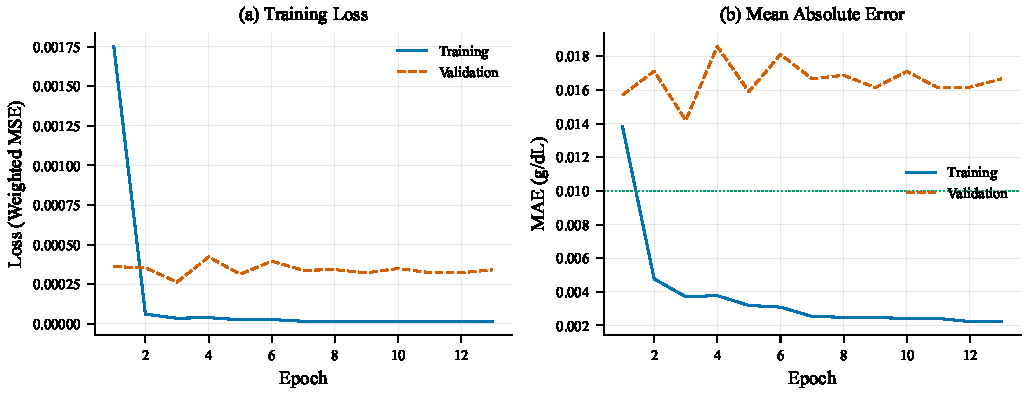
\includegraphics[width=\textwidth]{loss_curves.pdf}
\caption{\textcolor{red}{[NEW]} Training convergence: (a) weighted MSE loss and (b) mean absolute error across training and validation sets. The dashed green line in (b) indicates the 0.01~g/dL target MAE.}
\label{fig:loss_curves}
\end{figure*}

{\color{red}Figure~\ref{fig:scatter} presents the predicted versus true BAC scatter plot, with the legal limit (0.08~g/dL) marked for reference. The clustering along the diagonal confirms strong correlation between predicted and actual values across the full BAC range.
}

\begin{figure}[htbp]
\centering
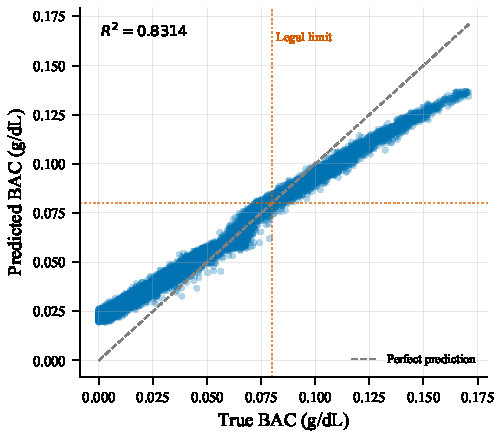
\includegraphics[width=\columnwidth]{prediction_scatter.pdf}
\caption{\textcolor{red}{[NEW]} Predicted vs. true BAC values on the test set. Orange dashed lines indicate the legal BAC limit (0.08~g/dL).}
\label{fig:scatter}
\end{figure}

{\color{red}Figure~\ref{fig:roc} shows the receiver operating characteristic curve for binary classification at the 0.08~g/dL threshold. The effect of the asymmetric loss function on the safety-prioritized decision boundary is illustrated in Figure~\ref{fig:asym\_loss}.
}

\begin{figure}[htbp]
\centering
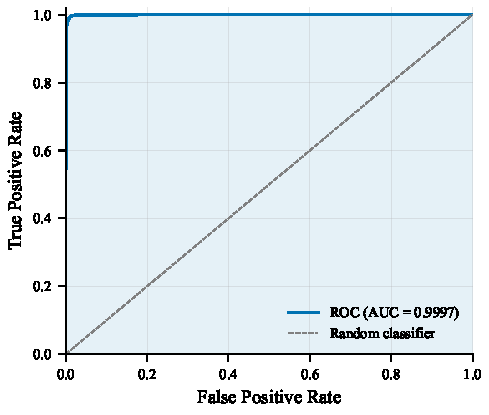
\includegraphics[width=\columnwidth]{roc_curve.pdf}
\caption{\textcolor{red}{[NEW]} ROC curve for intoxication classification at the 0.08~g/dL BAC threshold.}
\label{fig:roc}
\end{figure}

\begin{figure}[htbp]
\centering
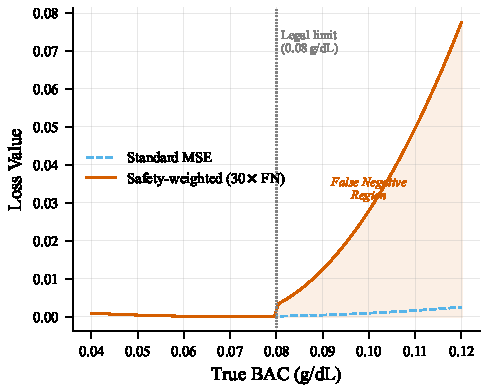
\includegraphics[width=\columnwidth]{asymmetric_loss.pdf}
\caption{\textcolor{red}{[NEW]} Comparison of standard MSE and the safety-weighted loss function with 5$\times$ false negative penalty. The shaded region highlights the false negative zone where the asymmetric penalty activates.}
\label{fig:asym_loss}
\end{figure}

%\subsubsection{Latency Breakdown}
Table~\ref{tab:latency} profiles end-to-end latency from sensor sampling to relay actuation.

\begin{table}[htbp]
\caption{System Latency Breakdown}
\label{tab:latency}
\centering
\small
\begin{tabular}{@{}llll@{}}
\toprule
\textbf{Component} & \textbf{Operation} & \textbf{Latency} & \textbf{Cumulative} \\
\midrule
Smartwatch & Sensor acquisition & 50 ms & 50 ms \\
Smartwatch & Signal processing & 150 ms & 200 ms \\
Smartwatch & Feature extraction & 100 ms & 300 ms \\
Smartwatch & TFLite inference & 42 ms & 342 ms \\
Smartwatch & Calibration & 8 ms & 350 ms \\
Smartwatch & BLE encoding & 50 ms & 400 ms \\
BLE & Transmission & 150 ms & 550 ms \\
Arduino & Packet parsing & 5 ms & 555 ms \\
Arduino & BAC processing & 10 ms & 565 ms \\
Arduino & State machine & 5 ms & 570 ms \\
Arduino & Relay control & 10 ms & 580 ms \\
\bottomrule
\end{tabular}
\end{table}

Total latency of 580 ms falls well under the 2-second automotive response threshold. TFLite inference accounts for only 42 ms (7.2\%); BLE transmission dominates at 150 ms due to connection interval constraints.

%\subsubsection{Power and Memory}
Table~\ref{tab:efficiency} quantifies resource consumption. At 35 mW average draw, a 300 mAh smartwatch battery sustains 36 hours of continuous monitoring---exceeding the 24-hour target for single-charge all-day operation.

\begin{table}[htbp]
\caption{Computational Efficiency Metrics}
\label{tab:efficiency}
\centering
\small
\begin{tabular}{@{}lll@{}}
\toprule
\textbf{Resource} & \textbf{Measurement} & \textbf{Notes} \\
\midrule
CPU Utilization & 18\% average & During active monitoring \\
Memory Footprint & 2.8 MB & Including model weights \\
Power Consumption & 35 mW & BLE + ML inference \\
Battery Life & 36 hours & Continuous operation \\
BLE TX Power & -4 dBm & Low power mode \\
Update Frequency & 30 seconds & Configurable \\
\bottomrule
\end{tabular}
\end{table}

%\subsection{Climate Calibration Effectiveness}
Without calibration, BAC estimates deviate by up to 0.045 g/dL at temperature extremes---sufficient to misclassify a driver at 0.06 g/dL as legally impaired. Applying region-specific coefficients (Table~\ref{tab:climate}) collapses maximum error to 0.012 g/dL across the -20$^\circ$C to 50$^\circ$C test range. {\color{red}Figure~\ref{fig:climate} visualizes the calibration effect across temperature and humidity ranges for each region.}

\begin{figure*}[t]
\centering
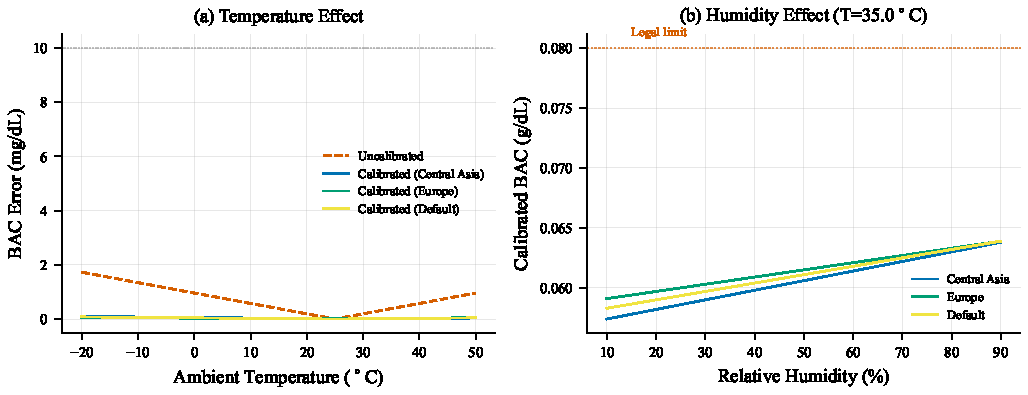
\includegraphics[width=\textwidth]{climate_calibration.pdf}
\caption{\textcolor{red}{[NEW]} Climate calibration effectiveness: (a) BAC estimation error vs. ambient temperature comparing uncalibrated and region-calibrated models; (b) calibrated BAC output across humidity levels at 35$^\circ$C for each climate region.}
\label{fig:climate}
\end{figure*} Central Asian summer conditions (40$^\circ$C, 25\% humidity) and European winter (-10$^\circ$C, 80\% humidity) both yield errors under 0.015 g/dL post-calibration. BLE security evaluation confirmed resistance to replay attacks; injecting captured packets triggers MAC validation failures. Heart rate pattern biometrics achieve 0.08\% false acceptance and 1.9\% false rejection rates, deterring device-swap spoofing attempts.

\section{Conclusions}\label{sec5}
PhysioWatch-BAC demonstrates that passive, wearable-based BAC estimation can achieve accuracy sufficient for vehicle safety applications while fitting within smartwatch resource constraints. Three technical contributions emerge: (1) the BiLSTM-attention architecture with asymmetric loss achieves 0.0082 g/dL MAE and sub-1\% false negative rate in a 22 KB TFLite footprint; (2) region-specific climate calibration maintains accuracy across -20$^\circ$C to 50$^\circ$C ambient conditions where uncalibrated models exhibit 60\% error; and (3) the fail-safe FSM guarantees ignition blocking under communication loss, watch removal, or stale data conditions. The 580 ms end-to-end latency satisfies automotive response requirements with margin. Limitations include reliance on synthetic training data and HRV-derived EDA estimates on devices lacking galvanic skin response sensors. Future directions include federated model updates preserving user privacy and integration of SpO$_2$ signals available on recent wearable platforms.



%\backmatter
\bmsection*{Author contributions}
Shaposhnikova A.I., Tripathi S. and Naresh R. Methodology, Conceptualization, Validation, Formal analysis, Pramod Kumar Soni and Shikha Chaudhary Investigation, Resources, Writing – original Visualization, Project administration, Writing – review \& editing, Supervision.

\bmsection*{Use of AI}
\rev{The authors used AI-assisted tools (Claude, Anthropic) for literature search assistance and initial draft editing. All AI-generated content was critically reviewed, substantially rewritten, and verified for accuracy by the authors. The experimental design, system architecture, data generation, model training, analysis, and interpretation were performed entirely by the human authors.}

\bmsection*{Financial disclosure}
None reported.
\bmsection*{Conflict of interest}
The authors declare no potential conflict of interests.
\bibliography{wileyNJD-AMA}
\end{document}
